\section{Introduction}
\label{sec:intro} 
\begin{figure}[t]
  \centering
  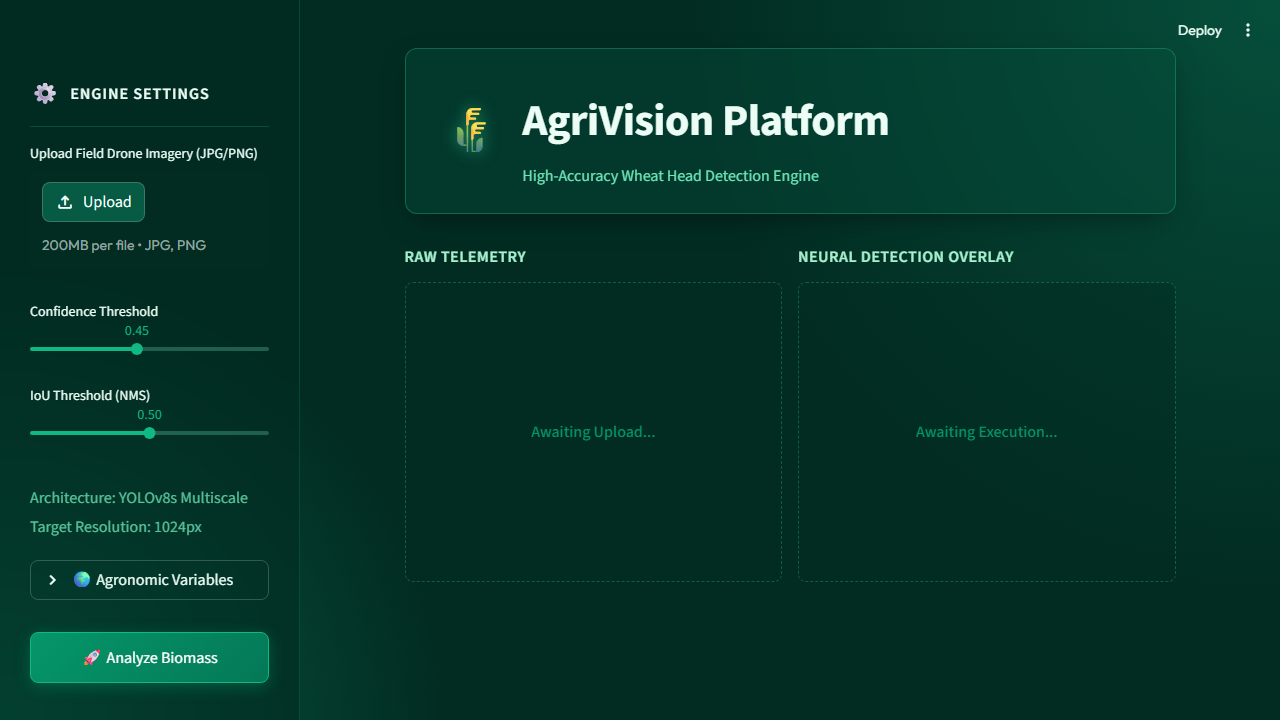
\includegraphics[width=\linewidth]{../docs/assets/dashboard_preview.png}
  
  \caption{The CropSense analytical interface. The system captures drone imagery, detects wheat heads with high fidelity via YOLOv8, and automatically calculates spatial uniformity and agronomic yield projections.}
  \label{fig:teaser}
\end{figure}

Securing a stable and abundant food supply is a paramount challenge for the 21st century. With fluctuating environmental conditions and a rapidly expanding global population, maximizing agricultural output while minimizing resource expenditure is no longer optional; it is imperative \cite{fao2023}. Wheat, as one of the world's most vital staple crops, requires accurate yield monitoring to ensure effective supply chain management and economic forecasting. Traditionally, agricultural professionals have relied on physical field scouting to estimate crop density. This method is inherently slow, highly subjective, and frequently leads to significant discrepancies between estimated and actual yields.

The advent of low-cost Unmanned Aerial Vehicles (UAVs) has revolutionized field monitoring by providing massive datasets of aerial imagery. However, the bottleneck has simply shifted from data collection to data analysis. While generic computer vision algorithms can identify objects within these images, they typically output disconnected bounding box coordinates that provide little immediate value to an agronomist. 

CropSense addresses this analytical bottleneck by providing a fully unified ecosystem for agricultural image processing. By harnessing the speed and accuracy of the YOLOv8 small architecture—fine-tuned extensively on the Global Wheat Detection dataset \cite{existing_study1}—our system reliably isolates individual wheat heads regardless of complex backgrounds, overlapping leaves, or harsh sunlight. 

Crucially, CropSense does not stop at mere detection. It incorporates a secondary mathematical framework that processes the coordinates of recognized crops to calculate actionable metrics. The system dynamically evaluates the spatial distribution of the crops to output a Coefficient of Variation (CV\%), providing a clear indicator of field health uniformity. Simultaneously, it computes an estimated yield in tons per hectare ($t/ha$). By automating the translation of raw pixels into executive-level agronomic data, CropSense fundamentally streamlines precision agriculture and empowers farmers to make data-driven decisions instantaneously.
